%%%%%%%%%%%%%%%%%%%%%%%%%%%%%%%%%%%%%%%%%
% University/School Laboratory Report
% LaTeX Template
% Version 3.1 (25/3/14)
%
% This template has been downloaded from:
% http://www.LaTeXTemplates.com
%
% Original author:
% Linux and Unix Users Group at Virginia Tech Wiki 
% (https://vtluug.org/wiki/Example_LaTeX_chem_lab_report)
%
% License:
% CC BY-NC-SA 3.0 (http://creativecommons.org/licenses/by-nc-sa/3.0/)
%
%%%%%%%%%%%%%%%%%%%%%%%%%%%%%%%%%%%%%%%%%

\documentclass[paper=letter, fontsize=11pt]{article}

% packages
\usepackage{fixltx2e}
\usepackage[pdftex]{graphicx}
\usepackage{color, wrapfig}
\usepackage{amsmath}  % required for some math elements 
\usepackage{fancyvrb, listings}  % for code verbatim and console outputs
\usepackage[margin=1in]{geometry}

\definecolor{dkgreen}{rgb}{0,0.6,0}
\definecolor{gray}{rgb}{0.5,0.5,0.5}
\definecolor{mauve}{rgb}{0.58,0,0.82}
\definecolor{black}{rgb}{0,0,0}

\lstset{frame=tb,
    language=R,
    aboveskip=3mm,
    belowskip=3mm,
    showstringspaces=false,
    columns=flexible,
    basicstyle={\small\ttfamily},
    numbers=none,
    numberstyle=\tiny\color{gray},
    keywordstyle=\color{blue},
    commentstyle=\color{dkgreen},
    stringstyle=\color{mauve},
    breaklines=true,
    breakatwhitespace=true,
    tabsize=4,
    escapechar={\?}
}

\newcommand{\n}{\newline\newline}

\setlength\parindent{0pt} % removes all indentation from paragraphs

% redefine \VerbatimInput
\RecustomVerbatimCommand{\VerbatimInput}{VerbatimInput}{
    fontsize=\footnotesize,
    frame=lines,  % top and bottom rule only
    framesep=2em,  % separation between frame and text
    rulecolor=\color{black},
    label=\fbox{\color{black}main.R},
    labelposition=topline,
}

%----------------------------------------------------------------------------------------
%	DOCUMENT INFORMATION
%----------------------------------------------------------------------------------------

\title{Project 3 \\ STAT 355}  % Title
\author{Sabbir \textsc{Ahmed}}  % Author name
\date{\today}  % Date for the report

\begin{document}

    \maketitle % Insert the title, author and date

    % ------------------------------ Part 1 ------------------------------

        \section{Part 1}
    \subsection{Question}
    An oceanographer wants to test, on the basis of a random sample of size 35, whether the average depth of the ocean in a certain area is 72.4 fathoms. At the 0.05 level of significance, what will the oceanographer decide if she gets a sample mean of 73.2? Assume the population standard deviation is 2.1.

    \subsection{Answer}
    The null hypothesis, $H_{0}$, claims the mean depth of the ocean in a certain area is 72.4, while the alternative hypothesis, $H_{a}$, says otherwise.

        \[ H_{0}: \mu = 72.4 \ vs \ H_{a}: \mu \neq 72.4 \]

    Since the population mean and standard deviation are known with a sample size of $n > 30$, the Z-score was calculated as follows:

        \begin{equation*}
    Z=\frac{\overline{X}-\mu}{\sfrac{\sigma}{\sqrt{n}}}
    =\frac{73.2-72.4}{\sfrac{2.1}{\sqrt{35}}}=2.2537
    \end{equation*}\newline

    The following snippet was used to generate the Z-test and its probability:
\begin{lstlisting}
    X <- 73.2
    mu <- 72.4
    sigma <- 2.1
    n <- 35
    alpha <- 0.05

    dumpComputation(X=X, mu=mu, sigma=sigma, n=n, 
        alpha=alpha, distType="Z", twoSided=TRUE, "part1")
\end{lstlisting}

    The test statistic was computed to be:

    \begin{equation*}
        Z_{1-\sfrac{0.05}{2}}=Z_{0.975}= 1.96 < 2.2537
    \end{equation*}

    The p-value was computed with the following snippet:
\begin{lstlisting}
    pScore <- 2 * (1 - (pnorm(score)))
    # 0.0242
\end{lstlisting}

    Since $Z_{\sfrac{\alpha}{2}} < Z$ and the p-score was under 0.05, the null hypothesis is rejected.


%         \subsection{Distribution}
%             Distribution of the data was plotted with a histogram using ggplot2 in Figure \ref{fig:hist1}.
% \begin{lstlisting}
%     ggplot() + aes(sampMeans) + 
%         geom_histogram(binwidth=0.1, color="black", fill="white") +
%         labs(y="Count", x="Sample Means")
% \end{lstlisting}

%             \begin{figure}[!h]
%                 \begin{center}
%                     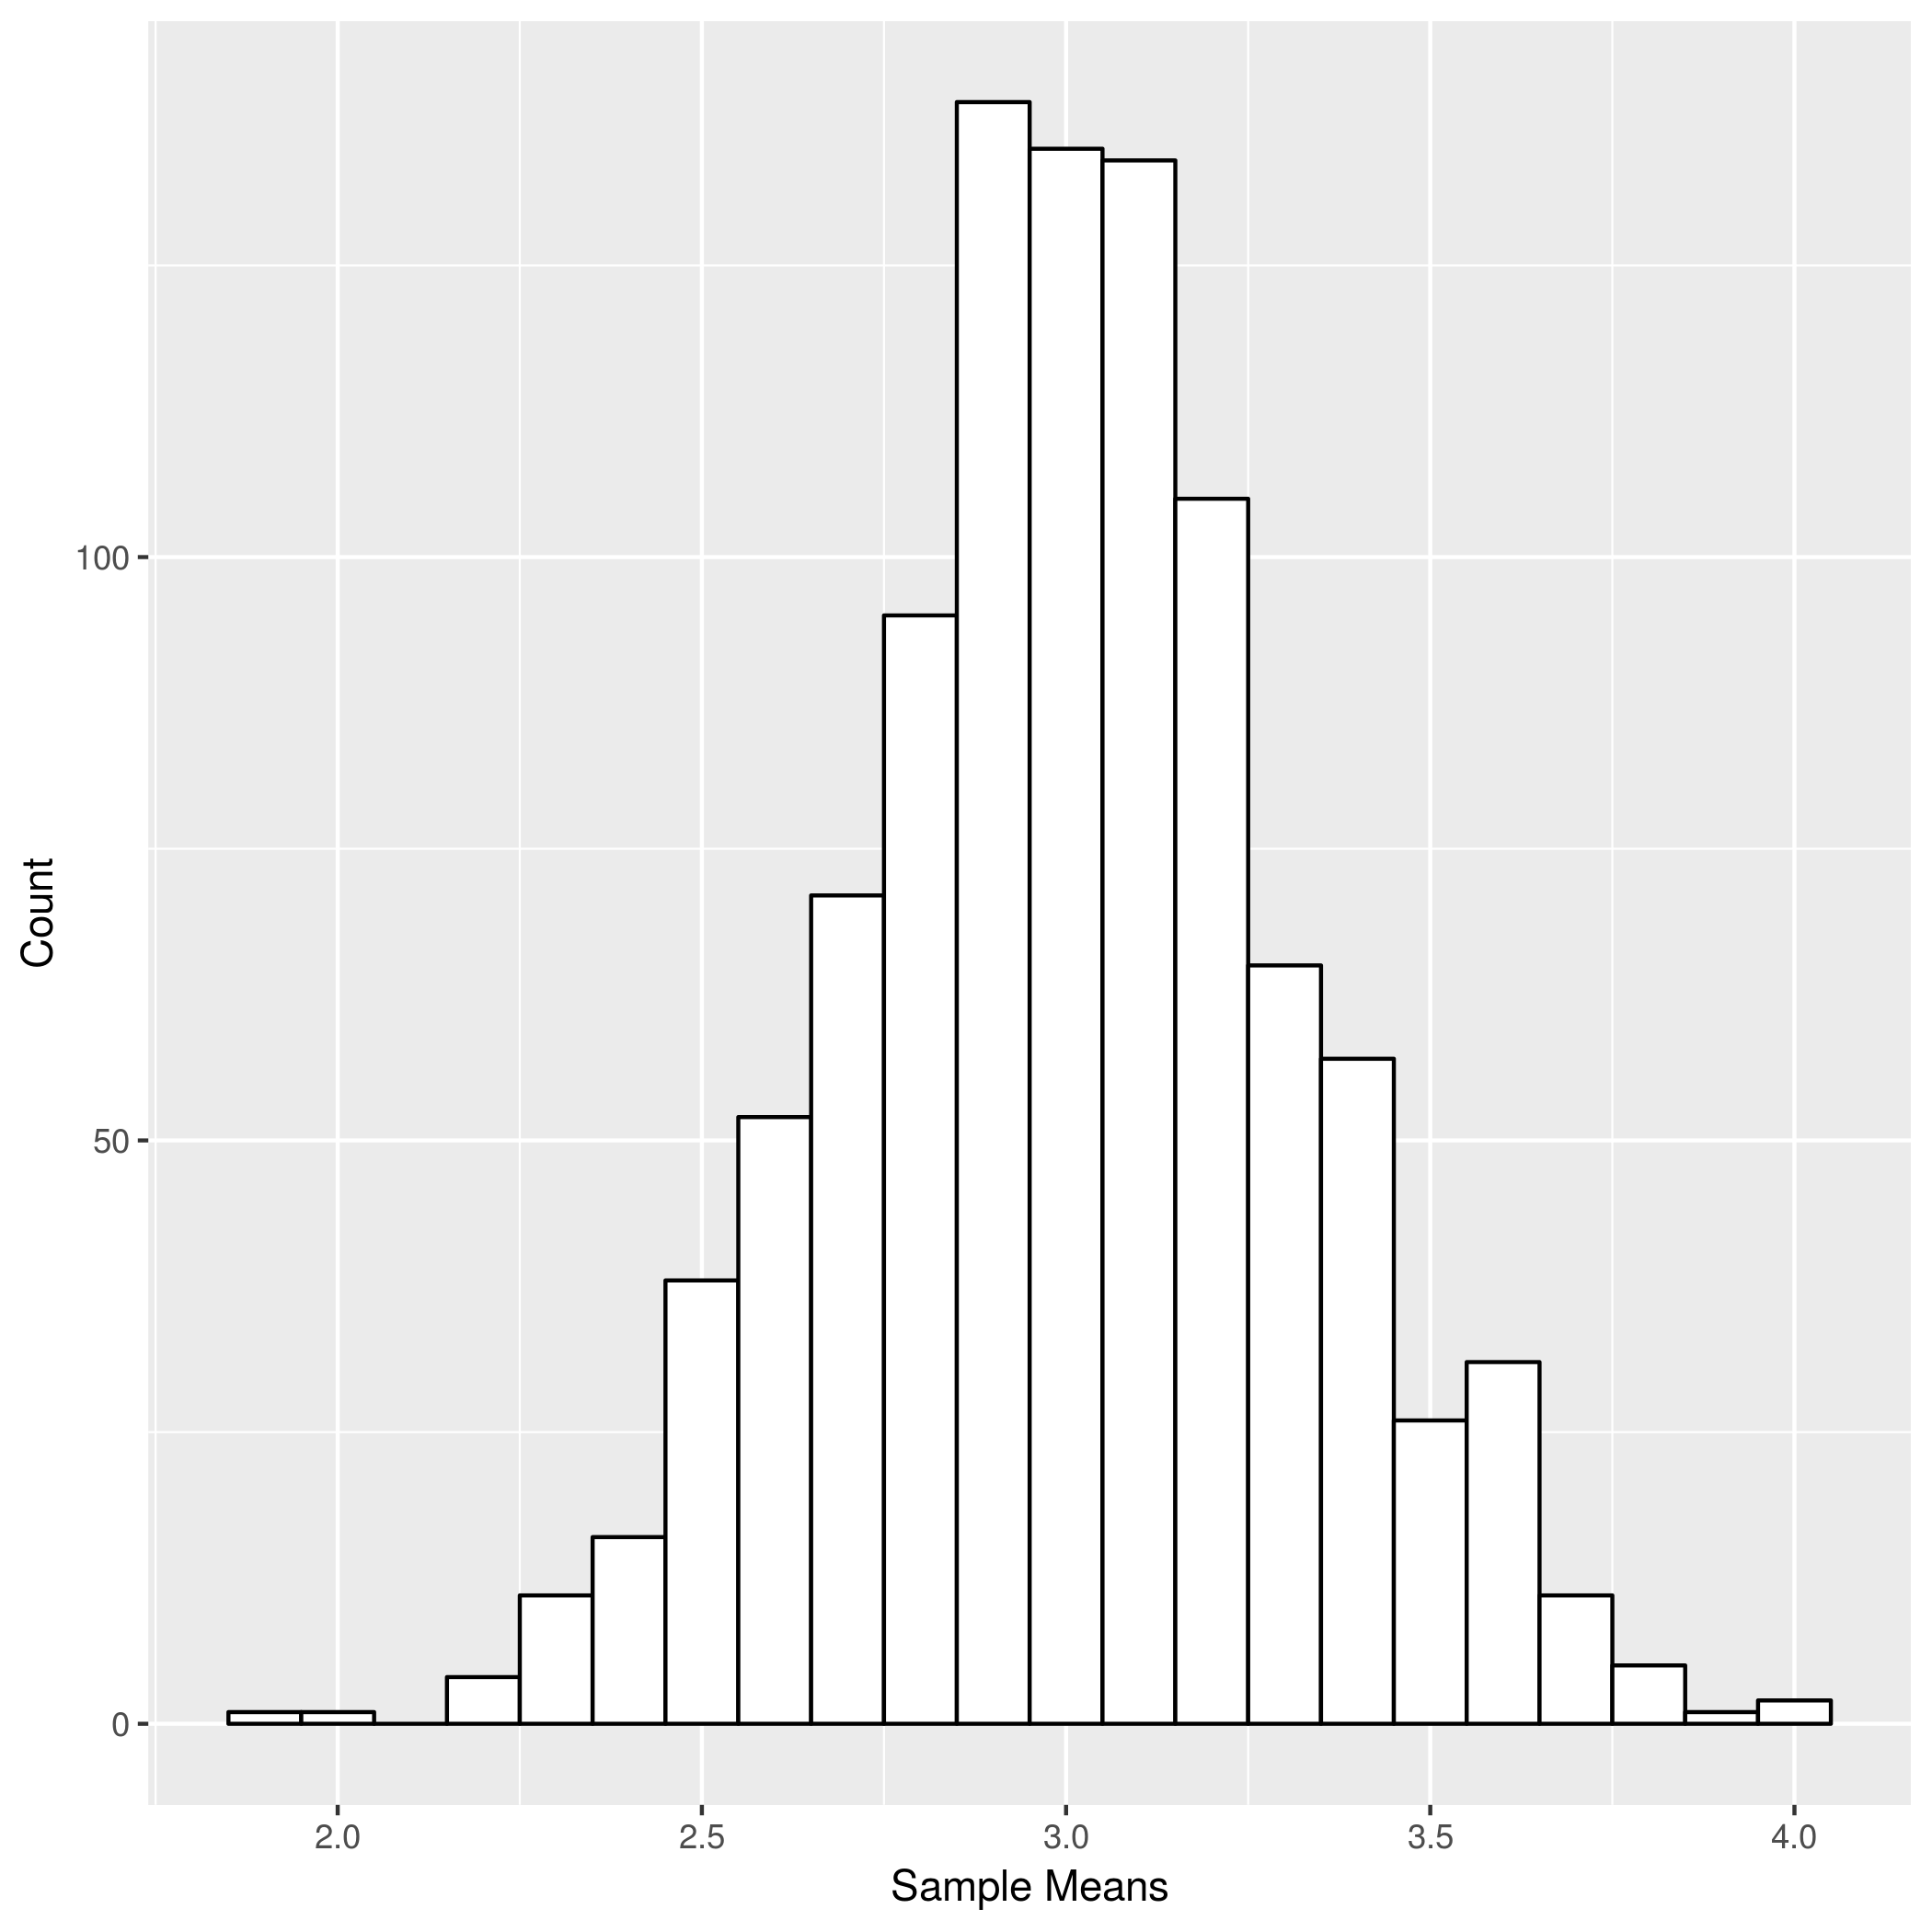
\includegraphics[width=0.5\textwidth]{figures/hist1.png}
%                     \caption{Histogram of the Generated Data} \label{fig:hist1}
%                 \end{center}
%             \end{figure}

%     \begin{thebibliography}{9}

%         \bibitem{wolfram}
%         Central Limit Theorem
%         \\\texttt{http://mathworld.wolfram.com/CentralLimitTheorem.html}

%     \end{thebibliography}

%     \clearpage
%     \newpage
%     \VerbatimInput{main.R}

\end{document}
